\documentclass{standalone}

\usepackage{tikz}
\usetikzlibrary{fit}

\begin{document}
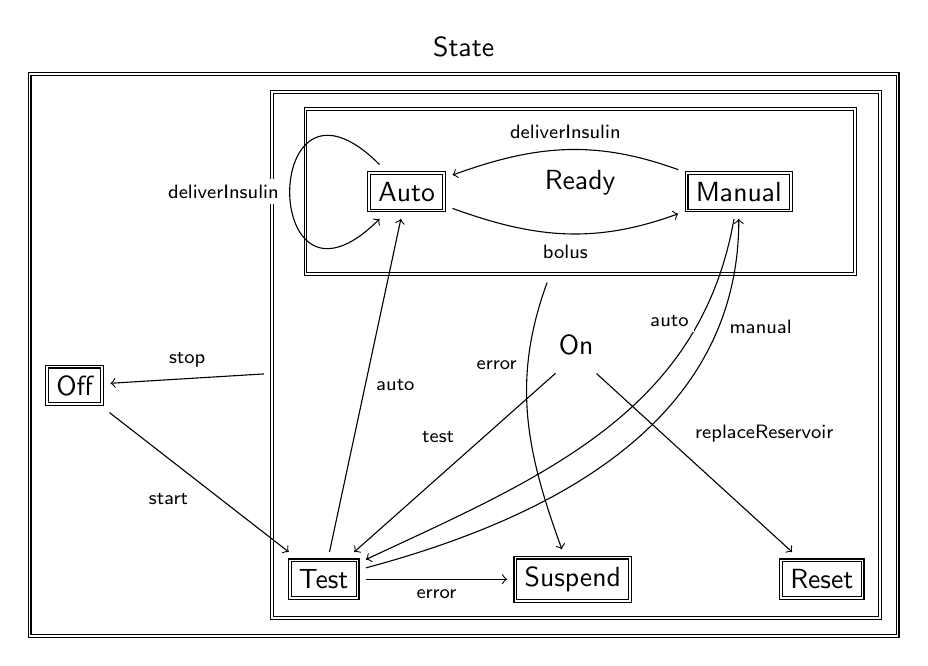
\begin{tikzpicture}[
  x=12em,
  y=7em,
  font=\sffamily,
  state/.style={
    draw,
    double,
    outer sep=3pt
  },
  trans/.style={
    font=\sffamily\scriptsize,
    fill=white,
    inner sep=2pt,
    outer sep=2pt
  },
  ->
  ]
  \node [state] (Off) at (0, 0) {Off};
  \node [state] (Auto) at (1, 1) {Auto};
  \node [state] (Manual) at (2, 1) {Manual};
  \node [state] (Ready) [fit={(Auto) (Manual)}, inner sep=20pt] {Ready};
  \node [state] (Test) at (0.75, -1) {Test};
  \node [state] (Suspend) at (1.5, -1) {Suspend};
  \node [state] (Reset) at (2.25, -1) {Reset};
  \node [state] (On) [fit={(Ready) (Test) (Suspend) (Reset)}] {On};
  \node [state] (State) [fit={(Off) (On)}, label={[above]:State}] {};

  \draw (Off) to node [trans, below left] {start} (Test);
  \draw (On) to node [trans, above] {stop} (Off);
  \draw [shorten <=1em] (On.center) to node [trans, above left] {test} (Test);
  \draw [shorten <=1em] (On.center) to node [trans, above right] {replaceReservoir} (Reset);
  \draw (Test) to node [trans, right] {auto} (Auto);
  \draw (Test) to [out=15, in=270] node [trans, pos=0.8, right] {manual} (Manual);
  \draw (Ready) to [out=250, in=110] node [trans, pos=0.3, left] {error} (Suspend);
  \draw (Test) to node [trans, below] {error} (Suspend);
  \draw (Auto) to [out=135, in=225, looseness=8] node [trans, left] {deliverInsulin} (Auto);
  \draw (Auto) to [out=340, in=200] node [trans, below] {bolus} (Manual);
  \draw (Manual) to [out=160, in=20] node [trans, above] {deliverInsulin} (Auto);
  \draw (Manual) to [out=260, in=25] node [trans, pos=0.2, left] {auto} (Test);
\end{tikzpicture}
\end{document}
